\chapter{Summarizing data}
\label{summarizingData}

\Comment{Do a search for "email" to see if it still appears
anywhere in this file. Do the same for the other chapters.}

In this chapter we will be introduced to techniques for exploring
and summarizing both numerical and categorical data.
We will consider two data sets that we first encountered
in Section~\ref{dataBasics}:
\begin{description}
\item[\data{loans}] We will consider loan data from
    10,000 Lending Club loans.
\item[\data{county}] We will consider several variables
    from the United States counties.
\end{description}
Each of these data sets provides several opportunities
for exploratory analyses.


%%%%%
\section[Examining numerical data]{Examining numerical data \sectionvideohref{youtube-Xm0PPtci3JE&list=PLkIselvEzpM6pZ76FD3NoCvvgkj_p-dE8}~\sectionslideshref{gdoc_os3_slides_1-6}}
\label{numericalData}

\Comment{Replace the \var{pop2010} variable with another example here.}
Outcomes of numerical variables are numbers on
which it is reasonable to perform basic arithmetic operations.
Below are the variables we will consider
For example, we'll encounter the \var{pop2010} variable,
which represents the populations of counties in 2010,
is numerical since we can sensibly discuss the difference
or ratio of the populations in two counties.
On the other hand, area codes and zip codes are not numerical,
but rather they are~categorical variables.

%In this section we will be introduced to techniques for exploring and summarizing numerical variables. The \data{email50} and \data{county} data sets from Section~\ref{dataBasics} provide rich opportunities for examples. Recall that outcomes of numerical variables are numbers on which it is reasonable to perform basic arithmetic operations. For example, the \var{pop2010} variable, which represents the populations of counties in 2010, is numerical since we can sensibly discuss the difference or ratio of the populations in two counties. On the other hand, area codes and zip codes are not numerical, but rather they are~categorical variables.


\subsection{Scatterplots for paired data}
\label{scatterPlots}

\index{data!email50|(}

\Comment{Ensure the referenced image still applies. If not, update.}
A \term{scatterplot} provides a case-by-case view of data
for two numerical variables.
In Figure~\vref{county_fed_spendVsPoverty}, a scatterplot
was used to examine how federal spending and poverty were
related in the \data{county} data set.
Another scatterplot is shown in Figure~\ref{loan50_amt_vs_income},
comparing the total income of a borrower (\var{total\_\hspace{0.3mm}income}) and the amount they borrowed
(\var{loan\_\hspace{0.3mm}amount}) for the \data{loan50} data set.
In any scatterplot, each point represents a single case.
Since there are 50 cases in \data{loan50},
there are 50 points in Figure~\ref{loan50_amt_vs_income}.

%\textC{\setlength{\captionwidth}{0.9\textwidth}}

\begin{figure}[h]
   \centering
   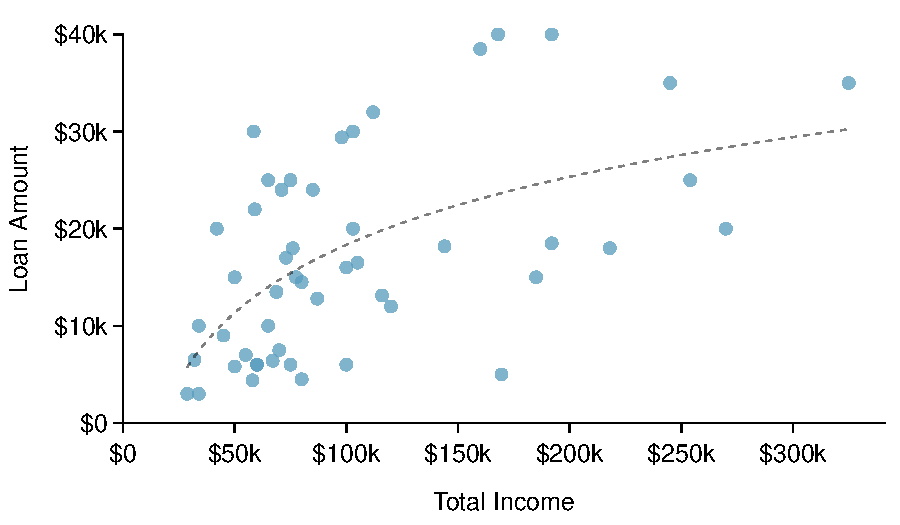
\includegraphics[width=0.8\textwidth]{ch_summarizing_data/figures/loan50_amt_vs_income/loan50_amt_vs_income}
   \caption{A scatterplot of \var{total\_\hspace{0.3mm}income}
       versus \var{loan\_\hspace{0.3mm}amount} for the
       \data{loan50} data set.
       A statistical model has also been fit to the data
       and is shown is a dashed line.}
   \label{loan50_amt_vs_income}
\end{figure}

%\textC{\setlength{\captionwidth}{\mycaptionwidth}}

Looking at Figure~\ref{loan50_amt_vs_income},
we see that there are many borrowers with an income below
\$100k (\$100,000) on the left side of the graph,
while there are a handful of borrowers with income above \$250k.
Additionally, the relationship appears to be \term{nonlinear},
where bigger loans seem to be associated with increased income,
but that it appears to taper off,
as shown by the dashed line.

\begin{exercise}
What do scatterplots reveal about the data,
and how might they be useful?\footnote{Answers may vary.
Scatterplots are helpful in quickly spotting associations
relating variables,
whether those associations come in the form of simple
trends or whether those relationships are more complex.}
\end{exercise}

%This is different from previous scatterplots we've seen, such as Figure~\vref{county_fed_spendVsPoverty} and Figure~\ref{email50LinesCharacters}, which show relationships that are very linear.

%\begin{figure}[h]
%   \centering
%   \includegraphics[width=0.8\textwidth]{ch_summarizing_data/figures/carsPriceVsWeight/carsPriceVsWeight}
%   \caption{A scatterplot of \var{price} versus \var{weight} for 54 cars.}
%   \label{carsPriceVsWeight}
%\end{figure}

\begin{exercise}
Describe two variables that would have a horseshoe-shaped
association in a scatterplot.\footnote{Consider the case
  where your vertical axis represents something ``good'' and
  your horizontal axis represents something that is only good
  in moderation.
  Health and water consumption fit this description: we require
  some water to survive, but consume too much and it becomes
  toxic and can kill a person.}
\end{exercise}

\subsection{Dot plots and the mean}
\label{dotPlot}

Sometimes two variables are one too many:
only one variable may be of interest.
In these cases, a dot plot provides the most basic of displays.
A~\term{dot plot} is a one-variable scatterplot;
an example using the loan amount of 50 loans
is shown in Figure~\ref{loan_amount_dot_plot}.
A stacked version of this dot plot is shown in
Figure~\ref{loan_amount_dot_plot_stacked}.

\begin{figure}[h]
   \centering
   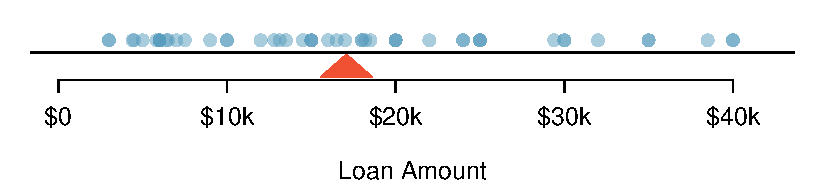
\includegraphics[width=0.76\textwidth]{ch_summarizing_data/figures/loan_amount_dot_plot/loan_amount_dot_plot}
   \caption{A dot plot of \var{loan\_\hspace{0.3mm}amount}
       for the \data{loan50} data set.
       The distribution's mean is shown as a red triangle.}
   \label{loan_amount_dot_plot}
\end{figure}

\begin{figure}[h]
   \centering
   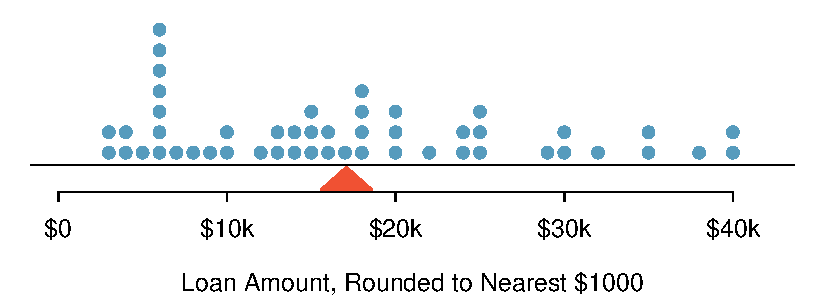
\includegraphics[width=0.76\textwidth]{ch_summarizing_data/figures/loan_amount_dot_plot/loan_amount_dot_plot_stacked}
   \caption{A stacked dot plot of \var{loan\_\hspace{0.3mm}amount}
       for the \data{loan50} data set. The~loan amounts have been
       rounded to the nearest \$1,000 in this plot, and the
       distribution's mean is shown as a red triangle.}
   \label{loan_amount_dot_plot_stacked}
\end{figure}

The \term{mean}, sometimes called the
\indexthis{average}{mean!average}, is a common way
to measure the center of a \term{distribution} of data.
To find the mean loan amount, we add up all the loan
amounts and divide by the number of loans:
\begin{align*}
\bar{x}
    = \frac{\text{\$7,500} + \text{\$25,000} +
        \cdots + \text{\$3,000}}{50}
    = \$17,083
% library(openintro); loan50$loan_amount[c(1, 2, 50)]; mean(loan50$loan_amount)
\end{align*}
The sample mean is often labeled $\bar{x}$.
The letter $x$ is being used as a generic placeholder
for the variable of interest, \var{loan\_\hspace{0.3mm}amount},
and the bar over on the $x$ communicates that the average
loan amount in the 50 loans was \$17,083.
It is useful to think of the mean as the balancing point
of the distribution, and it is shown as a triangle in Figures~\ref{loan_amount_dot_plot}
and~\ref{loan_amount_dot_plot_stacked}.

\begin{termBox}{\tBoxTitle{Mean}%
The sample mean of a numerical variable is computed as the sum
of all of the observations divided by the number of observations:
\begin{align*}
\bar{x} = \frac{x_1 + x_2 + \cdots + x_n}{n}
\end{align*}
where $x_1$, $x_2$, $\dots$, $x_n$ represent the $n$ observed values.}
\end{termBox}\marginpar[\raggedright\vspace{-8mm}

$n$\\\footnotesize sample size]{\raggedright\vspace{-8mm}

$n$\\\footnotesize sample size}\vspace{-2mm}

\begin{exercise}
Examine the equation for the mean.
What does $x_1$ correspond to? And $x_2$?
Can you infer a general meaning to what $x_i$
might represent?\footnote{$x_1$ corresponds to the
  loan amount in the first loan in the sample (\$7,500),
  $x_2$ to the second loan's amount (\$25,000),
  and $x_i$ corresponds to the loan amount in the
  $i^{th}$ loan in the data set.}
\end{exercise}

\begin{exercise}
What was $n$ in this sample of
loans?\footnote{The sample size was $n = 50$.}
\end{exercise}

The \data{loan50} data set represents a sample from
a larger population of loans that were \Comment{add details}.
We could compute a mean for this population in the same way
as the sample mean.
However, the population mean has a special label: $\mu$.
\index{Greek!mu@mu ($\mu$)}
The symbol $\mu$ is the Greek letter \emph{mu} and represents
the average of all observations in the population.
Sometimes a subscript, such as $_x$,
is used to represent which variable the population mean
refers to, e.g. $\mu_x$.

\begin{example}{The average loan amount across all loans
  in the population can be estimated using the sample data.
  Based on the sample of 50 loans,
  what would be a reasonable estimate of $\mu_x$,
  the mean number of characters in all emails in the
  \data{loan} data set?
  (Recall that \data{loan50} is a sample from \data{loan}.)}
The sample mean, \$17,083, may provide a reasonable estimate
of $\mu_x$.
While this number will not be perfect,
it provides a \emph{point estimate} of the population mean.
In Chapter~\ref{foundationsForInference} and beyond,
we will develop tools to characterize the accuracy
of point estimates, and we will find that point estimates
based on larger samples tend to be more accurate than
those based on smaller samples.
\end{example}

\begin{example}{We might like to compute the average income per person in the US. To do so, we might first think to take the mean of the per capita incomes across the 3,143 counties in the \data{county} data set. What would be a better approach?} \label{wtdMeanOfIncome}
The \data{county} data set is special in that each county actually represents many individual people. If we were to simply average across the \var{income} variable, we would be treating counties with 5,000 and 5,000,000 residents equally in the calculations. Instead, we should compute the total income for each county, add up all the counties' totals, and then divide by the number of people in all the counties. If we completed these steps with the \data{county} data, we would find that the per capita income for the US is \$27,348.43. Had we computed the \emph{simple} mean of per capita income across counties, the result would have been just \$22,504.70!
\end{example}

Example~\ref{wtdMeanOfIncome} used what is called a \term{weighted mean}\index{mean!weighted mean}, which will not be a key topic in this textbook. However, we have provided an online supplement on weighted means for interested readers:
\begin{center}
\oiRedirect{textbook-weighted_mean_supplement}{www.openintro.org/d?f=wtdmean}
\end{center}

\subsection{Histograms and shape}
\label{histogramsAndShape}

Dot plots show the exact value for each observation. This is useful for small data sets, but they can become hard to read with larger samples. Rather than showing the value of each observation, we prefer to think of the value as belonging to a \emph{bin}. For example, in the \data{email50} data set, we create a table of counts for the number of cases with character counts between 0 and 5,000, then the number of cases between 5,000 and 10,000, and so on. Observations that fall on the boundary of a bin (e.g. 5,000) are allocated to the lower bin. This tabulation is shown in Figure~\ref{binnedNumCharTable}. These binned counts are plotted as bars in Figure~\ref{email50NumCharHist} into what is called a \term{histogram}, which resembles the stacked dot plot shown in Figure~\ref{loan_amount_dot_plot_stacked}.

\begin{figure}[ht]
\centering\small
\begin{tabular}{l ccc ccc ccc c}
  \hline
Characters & \\
(in thousands) & \raisebox{1.5ex}[0pt]{0-5} & \raisebox{1.5ex}[0pt]{5-10} & \raisebox{1.5ex}[0pt]{10-15} & \raisebox{1.5ex}[0pt]{15-20} & \raisebox{1.5ex}[0pt]{20-25} & \raisebox{1.5ex}[0pt]{25-30} & \raisebox{1.5ex}[0pt]{$\cdots$} & \raisebox{1.5ex}[0pt]{55-60} & \raisebox{1.5ex}[0pt]{60-65} \\
  \hline
Count & 19 & 12 & 6 & 2 & 3 & 5 & $\cdots$ & 0 & 1 \\
  \hline
\end{tabular}
\caption{The counts for the binned \var{num\_\hspace{0.3mm}char} data.}
\label{binnedNumCharTable}
\end{figure}

\begin{figure}[bth]
   \centering
   \includegraphics[width=0.82\textwidth]{ch_summarizing_data/figures/email50NumCharHist/email50NumCharHist}
   \caption{A histogram of \var{num\_\hspace{0.3mm}char}. This distribution is very strongly skewed to the right.\index{skew!example: very strong}}
   \label{email50NumCharHist}
\end{figure}

Histograms provide a view of the \term{data density}. Higher bars represent where the data are relatively more common. For instance, there are many more emails with fewer than 20,000 characters than emails with at least 20,000 in the data set. The bars make it easy to see how the density of the data changes relative to the number of characters.

Histograms are especially convenient for describing the shape of the data distribution\label{shapeFirstDiscussed}. Figure~\ref{email50NumCharHist} shows that most emails have a relatively small number of characters, while fewer emails have a very large number of characters. When data trail off to the right in this way and have a longer right \hiddenterm{tail}\index{skew!tail}, the shape is said to be \termsub{right skewed}{skew!right skewed}.\footnote{Other ways to describe data that are skewed to the right: \termni{skewed to the right}, \termni{skewed to the high end}, or \termni{skewed to the positive end}.}

Data sets with the reverse characteristic -- a long, thin tail to the left -- are said to be \termsub{left skewed}{skew!left skewed}. We also say that such a distribution has a long left tail. Data sets that show roughly equal trailing off in both directions are called \term{symmetric}.\index{skew!symmetric}

\begin{termBox}{\tBoxTitle{Long tails to identify skew}%
When data trail off in one direction, the distribution has a \term{long tail}. \index{skew!long tail|textbf} If a distribution has a long left tail, it is left skewed. If a distribution has a long right tail, it is right skewed.}
\end{termBox}

\begin{exercise}
Take a look at the dot plots in Figures~\ref{loan_amount_dot_plot} and~\ref{loan_amount_dot_plot_stacked}. Can you see the skew in the data? Is it easier to see the skew in this histogram or the dot plots?\footnote{The skew is visible in all three plots, though the flat dot plot is the least useful. The stacked dot plot and histogram are helpful visualizations for identifying skew.}
\end{exercise}

\begin{exercise}
Besides the mean (since it was labeled), what can you see in the dot plots that you cannot see in the histogram?\footnote{Character counts for individual emails.}
\end{exercise}

In addition to looking at whether a distribution is skewed or symmetric, histograms can be used to identify modes. A \term{mode} is represented by a prominent peak in the distribution.\footnote{Another definition of mode, which is not typically used in statistics, is the value with the most occurrences. It is common to have \emph{no} observations with the same value in a data set, which makes this other definition useless for many real data sets.} There is only one prominent peak in the histogram of \var{num\_\hspace{0.3mm}char}.

Figure~\ref{singleBiMultiModalPlots} shows histograms that have one, two, or three prominent peaks. Such distributions are called \termsub{unimodal}{modality!unimodal}, \termsub{bimodal}{modality!bimodal}, and \termsub{multimodal}{modality!multimodal}, respectively. Any distribution with more than 2 prominent peaks is called multimodal. Notice that there was one prominent peak in the unimodal distribution with a second less prominent peak that was not counted since it only differs from its neighboring bins by a few observations.

\begin{figure}[h]
   \centering
   \includegraphics[width=0.9\textwidth]{ch_summarizing_data/figures/singleBiMultiModalPlots/singleBiMultiModalPlots}
   \caption{Counting only prominent peaks, the distributions are (left to right) unimodal, bimodal, and multimodal. Note that we've said the left plot is unimodal intentionally. This is because we are counting \emph{prominent} peaks, not just any peak. See the Tip box for more thoughts.}
   \label{singleBiMultiModalPlots}
\end{figure}

\begin{exercise}
Figure~\ref{email50NumCharHist} reveals only one prominent mode in the number of characters. Is the distribution unimodal, bimodal, or multimodal?\footnote{Unimodal. Remember that \emph{uni} stands for 1 (think \emph{uni}cycles). Similarly, \emph{bi} stands for~2 (think \emph{bi}cycles). (We're hoping a \emph{multicycle} will be invented to complete this analogy.)}
\end{exercise}

\begin{exercise}
Height measurements of young students and adult teachers at a K-3 elementary school were taken. How many modes would you anticipate in this height data set?\footnote{There might be two height groups visible in the data set: one of the students and one of the adults. That is, the data are probably bimodal.}
\end{exercise}

\begin{tipBox}{\tipBoxTitle{Looking for modes}
Looking for modes isn't about finding a clear and correct answer about the number of modes in a distribution, which is why \emph{prominent} is not rigorously defined in this book. The important part of this examination is to better understand your data and how it might be structured.}
\end{tipBox}


\subsection{Variance and standard deviation}
\label{variability}

The mean was introduced as a method to describe the center of a data set, but the \indexthis{variability}{variability} in the data is also important. Here, we introduce two measures of variability: the variance and the standard deviation. Both of these are very useful in data analysis, even though their formulas are a bit tedious to calculate by hand. The standard deviation is the easier of the two to understand, and it roughly describes how far away the typical observation is from the mean.

We call the distance of an observation from its mean its \term{deviation}. Below are the deviations for the $1^{st}_{}$, $2^{nd}_{}$, $3^{rd}$, and $50^{th}_{}$ observations in the \var{num\_\hspace{0.3mm}char} variable. For computational convenience, the number of characters is listed in the thousands and rounded to the first decimal.
\begin{align*}
x_1^{}-\bar{x} &= 21.7 - 11.6 = 10.1 \hspace{5mm}\text{ } \\
x_2^{}-\bar{x} &= 7.0 - 11.6 = -4.6 \\
x_3^{}-\bar{x} &= 0.6 - 11.6 = -11.0 \\
			&\ \vdots \\
x_{50}^{}-\bar{x} &= 15.8 - 11.6 = 4.2
\end{align*}
% library(openintro); d <- email50$num_char; round(mean(d),1); d[c(1,2,3,50)]; d[c(1,2,3,50)] - round(mean(d),1); (d[c(1,2,3,50)] - round(mean(d)))^2; sum((d - round(mean(d)))^2)/49; sqrt(sum((d - round(mean(d)))^2)/49); var(d); sd(d)
If we square these deviations and then take an average, the result is about equal to the sample \term{variance}\label{varianceIsDefined}, denoted by $s_{}^2$\marginpar[\raggedright$s^2_{}$\\\footnotesize sample variance]{\raggedright$s^2_{}$\\\footnotesize sample variance}:
\begin{align*}
s_{}^2 &= \frac{10.1_{}^2 + (-4.6)_{}^2 + (-11.0)_{}^2 + \cdots + 4.2_{}^2}{50-1} \\
	&= \frac{102.01 + 21.16 + 121.00 + \cdots + 17.64}{49} \\
	&= 172.44
\end{align*}
We divide by $n-1$, rather than dividing by $n$, when computing the variance; you need not worry about this mathematical nuance for the material in this textbook. Notice that squaring the deviations does two things. First, it makes large values much larger, seen by comparing $10.1^2$, $(-4.6)^2$, $(-11.0)^2$, and $4.2^2$. Second, it gets rid of any negative signs.

The \term{standard deviation} is defined as the square root of the variance:
$$s=\sqrt{172.44} = 13.13$$
\marginpar[\raggedright\vspace{-10mm}

$s$\\\footnotesize sample standard deviation]{\raggedright\vspace{-10mm}

$s$\\\footnotesize sample standard deviation
}\index{s@$s$}The standard deviation of the number of characters in an email is about 13.13 thousand. A subscript of $_x$ may be added to the variance and standard deviation, i.e. $s_x^2$ and $s_x^{}$, as a reminder that these are the variance and standard deviation of the observations represented by $x_1^{}$, $x_2^{}$, ..., $x_n^{}$. The $_{x}$ subscript is usually omitted when it is clear which data the variance or standard deviation is referencing.

\begin{termBox}{\tBoxTitle{Variance and standard deviation}
The variance is roughly the average squared distance from the mean. The standard deviation is the square root of the variance. The standard deviation is useful when considering how close the data are to the mean.}
\end{termBox}

Formulas and methods used to compute the variance and standard deviation for a population are similar to those used for a sample.\footnote{The only difference is that the population variance has a division by $n$ instead of $n-1$.} However, like the mean, the population values have special symbols: $\sigma_{}^2$\marginpar[\raggedright$\sigma_{}^2$\\\footnotesize population variance\\ \hspace{2mm}]{\raggedright$\sigma_{}^2$\\\footnotesize population variance\\ \hspace{2mm}} for the variance and $\sigma$\marginpar[\raggedright$\sigma$\\\footnotesize population standard deviation\\ \hspace{2mm}]{\raggedright$\sigma$\\\footnotesize population standard deviation\\ \hspace{2mm}} for the standard deviation. The symbol $\sigma$ \index{Greek!sigma@sigma ($\sigma$)} is the Greek letter \emph{sigma}.


\begin{figure}
\centering
\includegraphics[width=\mycaptionwidth]{ch_summarizing_data/figures/sdAsRuleForEmailNumChar/sdAsRuleForEmailNumChar}
\caption{In the \var{num\_\hspace{0.3mm}char} data, 41 of the 50 emails (82\%) are within 1~standard deviation of the mean, and 47 of the 50 emails (94\%) are within 2 standard deviations. Usually about 70\% of the data are within 1 standard deviation of the mean and 95\% are within 2 standard deviations, though this rule of thumb is less accurate for skewed data, as shown in this example.}
\label{sdAsRuleForEmailNumChar}
\end{figure}

\begin{tipBox}{\tipBoxTitle{standard deviation describes variability}
Focus on the conceptual meaning of the standard deviation as a descriptor of variability rather than the formulas. Usually 70\% of the data will be within one standard deviation of the mean and about 95\% will be within two standard deviations. However, as seen in Figures~\ref{sdAsRuleForEmailNumChar} and~\ref{severalDiffDistWithSdOf1}, these percentages are not strict rules.}
\end{tipBox}

\begin{figure}
\centering
\includegraphics[width=0.64\textwidth]{ch_summarizing_data/figures/severalDiffDistWithSdOf1/severalDiffDistWithSdOf1}
\caption{Three very different population distributions with the same mean $\mu=0$ and standard deviation $\sigma=1$.}
\label{severalDiffDistWithSdOf1}
\end{figure}

\begin{exercise}
On page~\pageref{shapeFirstDiscussed}, the concept of shape of a distribution was introduced. A good description of the shape of a distribution should include modality and whether the distribution is symmetric or skewed to one side. Using Figure~\ref{severalDiffDistWithSdOf1} as an example, explain why such a description is important.\footnote{Figure~\ref{severalDiffDistWithSdOf1} shows three distributions that look quite different, but all have the same mean, variance, and standard deviation. Using modality, we can distinguish between the first plot (bimodal) and the last two (unimodal). Using skewness, we can distinguish between the last plot (right skewed) and the first two. While a picture, like a histogram, tells a more complete story, we can use modality and shape (symmetry/skew) to characterize basic information about a~distribution.}
\end{exercise}

\begin{example}{Describe the distribution of the \var{num\_\hspace{0.3mm}char} variable using the histogram in Figure~\ref{email50NumCharHist}. The description should incorporate the center, variability, and shape of the distribution, and it should also be placed in context: the number of characters in emails. Also note any especially unusual cases.}
The distribution of email character counts is unimodal and very strongly skewed to the high end. Many of the counts fall near the mean at 11,600, and most fall within one standard deviation (13,130) of the mean. There is one exceptionally long email with about 65,000 characters.
\end{example}

In practice, the variance and standard deviation are sometimes used as a means to an end, where the ``end'' is being able to accurately estimate the uncertainty associated with a sample statistic. For example, in Chapter~\ref{foundationsForInference} we will use the variance and standard deviation to assess how close the sample mean is to the population mean.

\subsection{Box plots, quartiles, and the median}

A \term{box plot} summarizes a data set using five statistics while also plotting unusual observations. Figure~\ref{boxPlotLayoutNumVar} provides a vertical dot plot alongside a box plot of the \var{num\_\hspace{0.3mm}char} variable from the \data{email50} data set.

\begin{figure}[h]
   \centering
   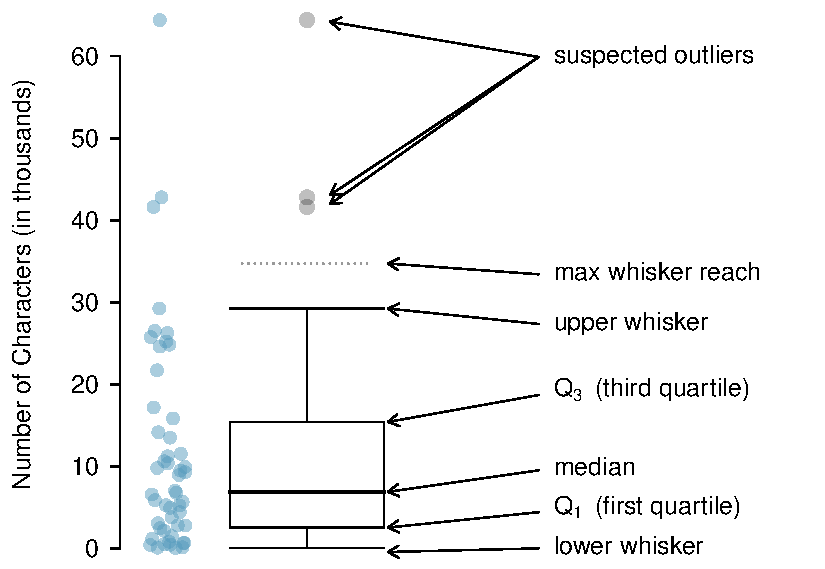
\includegraphics[width=0.86\mycaptionwidth]{ch_summarizing_data/figures/boxPlotLayoutNumVar/boxPlotLayoutNumVar}
   \caption{A vertical dot plot next to a labeled box plot for the number of characters in 50 emails. The median (6,890), splits the data into the bottom 50\% and the top 50\%.}
   \label{boxPlotLayoutNumVar}
\end{figure}

The first step in building a box plot is drawing a dark line denoting the \term{median}, which splits the data in half. Figure~\ref{boxPlotLayoutNumVar} shows 50\% of the data falling below the median and other 50\% falling above the median. There are 50 character counts in the data set (an even number) so the data are perfectly split into two groups of~25. We take the median in this case to be the average of the two observations closest to the $50^{th}$ percentile: $(\text{6,768} + \text{7,012}) / 2 = \text{6,890}$. When there are an odd number of observations, there will be exactly one observation that splits the data into two halves, and in such a case that observation is the median (no average needed).

\begin{termBox}{\tBoxTitle{Median: the number in the middle}
If the data are ordered from smallest to largest, the \term{median} is the observation right in the middle. If there are an even number of observations, there will be two values in the middle, and the median is taken as their average.}
\end{termBox}

The second step in building a box plot is drawing a rectangle to represent the middle 50\% of the data. The total length of the box, shown vertically in Figure~\ref{boxPlotLayoutNumVar}, is called the \term{interquartile range} (\hiddenterm{IQR}, for short). It, like the standard deviation, is a measure of \indexthis{variability}{variability} in data. The more variable the data, the larger the standard deviation and~IQR. The two boundaries of the box are called the \term{first quartile} \index{quartile!first quartile} (the $25^{th}$ \hiddenterm{percentile}, i.e. 25\% of the data fall below this value) and the \term{third quartile} \index{quartile!third quartile} (the $75^{th}$ percentile), and these are often labeled $Q_1$ \index{Q$_1$} and $Q_3$\index{Q$_3$}, respectively.

\begin{termBox}{\tBoxTitle{Interquartile range (IQR)}
The IQR\index{interquartile range} is the length of the box in a box plot. It is computed as
\begin{eqnarray*}
IQR = Q_3 - Q_1
\end{eqnarray*}
where $Q_1$ and $Q_3$ are the $25^{th}$ and $75^{th}$ percentiles.}
\end{termBox}

\begin{exercise}
What percent of the data fall between $Q_1$ and the median? What percent is between the median and $Q_3$?\footnote{Since $Q_1$ and $Q_3$ capture the middle 50\% of the data and the median splits the data in the middle, 25\% of the data fall between $Q_1$ and the median, and another 25\% falls between the median and $Q_3$.}
\end{exercise}

Extending out from the box, the \term{whiskers} attempt to capture the data outside of the box, however, their reach is never allowed to be more than $1.5\times IQR$.\footnote{While the choice of exactly 1.5 is arbitrary, it is the most commonly used value for box plots.} They capture everything within this reach. In Figure~\ref{boxPlotLayoutNumVar}, the upper whisker does not extend to the last three points, which is beyond $Q_3 + 1.5\times IQR$, and so it extends only to the last point below this limit. The lower whisker stops at the lowest value, 33, since there is no additional data to reach; the lower whisker's limit is not shown in the figure because the plot does not extend down to $Q_1 - 1.5\times IQR$. In a sense, the box is like the body of the box plot and the whiskers are like its arms trying to reach the rest of the data.

Any observation that lies beyond the whiskers is labeled with a dot. The purpose of labeling these points -- instead of just extending the whiskers to the minimum and maximum observed values -- is to help identify any observations that appear to be unusually distant from the rest of the data. Unusually distant observations are called \termsub{outliers}{outlier}. In this case, it would be reasonable to classify the emails with character counts of 41,623, 42,793, and 64,401 as outliers since they are numerically distant from most of the data.

\begin{termBox}{\tBoxTitle{Outliers are extreme}
An \term{outlier} is an observation that appears extreme relative to the rest of the data.}
\end{termBox}


\begin{tipBox}{\tipBoxTitle{Why it is important to look for outliers}
Examination of data for possible outliers serves many useful purposes, including\vspace{-2mm}
\begin{enumerate}
\setlength{\itemsep}{0mm}
\item Identifying \indexthis{strong skew}{skew!example: strong} in the distribution.
\item Identifying data collection or entry errors. For instance, we re-examined the email purported to have 64,401 characters to ensure this value was accurate.
\item Providing insight into interesting properties of the data.\vspace{0.5mm}
\end{enumerate}}
\end{tipBox}

\begin{exercise}
The observation 64,401, a suspected outlier, was found to be an accurate observation. What would such an observation suggest about the nature of character counts in emails?\footnote{That occasionally there may be very long emails.}\end{exercise}

\begin{exercise}
Using Figure~\ref{boxPlotLayoutNumVar}, estimate the following values for \var{num\_\hspace{0.3mm}char} in the \data{email50} data set: (a) $Q_1$, (b) $Q_3$, and (c) IQR.\footnote{These visual estimates will vary a little from one person to the next: $Q_1=$ 3,000, $Q_3=$ 15,000, $\text{IQR}=Q_3 - Q_1 = $ 12,000. (The true values: $Q_1=$ 2,536, $Q_3=$ 15,411, $\text{IQR} = $ 12,875.)}
\end{exercise}

\CalculatorVideos{how to create statistical summaries and box plots}


\subsection{Robust statistics}

How are the \indexthis{sample statistics}{sample statistic} of the \data{num\_\hspace{0.3mm}char} data set affected by the observation, 64,401? What would have happened if this email wasn't observed? What would happen to these \indexthis{summary statistics}{summary statistic} if the observation at 64,401 had been even larger, say 150,000? These scenarios are plotted alongside the original data in Figure~\ref{email50NumCharDotPlotRobustEx}, and sample statistics are computed under each scenario in Figure~\ref{robustOrNotTable}.

\begin{figure}[ht]
\centering
\includegraphics[width=\textwidth]{ch_summarizing_data/figures/email50NumCharDotPlotRobustEx/email50NumCharDotPlotRobustEx}
\caption{Dot plots of the original character count data and two modified data sets.}
\label{email50NumCharDotPlotRobustEx}
\end{figure}

\begin{figure}[ht]
\centering
\begin{tabular}{l c cc c cc}
  \hline
& \hspace{0mm} & \multicolumn{2}{c}{\bf robust} & \hspace{2mm} & \multicolumn{2}{c}{\bf not robust} \\
scenario && median & IQR && $\bar{x}$ & $s$ \\ 
  \hline
original \var{num\_\hspace{0.3mm}char} data 	&& 6,890 & 12,875 && 11,600 & 13,130 \\
% library(openintro); data(email50); d <- email50$num_char; median(d); diff(quantile(d, c(0.25,0.75))); mean(d); sd(d)
drop 64,401 observation		&& 6,768 & 11,702 && 10,521 & 10,798 \\
% library(openintro); data(email50); d <- email50$num_char; d <- d[-which.max(d)]; median(d); diff(quantile(d, c(0.25,0.75))); mean(d); sd(d)
move 64,401 to 150,000		&& 6,890 & 12,875 && 13,310 & 22,434 \\
% library(openintro); data(email50); d <- email50$num_char; d[which.max(d)] <- 100000; median(d); diff(quantile(d, c(0.25,0.75))); mean(d); sd(d)
   \hline
\end{tabular}
\caption{A comparison of how the median, IQR, mean ($\bar{x}$), and standard deviation ($s$) change when extreme observations are present.}
\label{robustOrNotTable}
\end{figure}

\begin{exercise} \label{numCharWhichIsMoreRobust}
(a) Which is more affected by extreme observations, the mean or median? Figure~\ref{robustOrNotTable} may be helpful. (b) Is the standard deviation or IQR more affected by extreme observations?\footnote{(a) Mean is affected more. (b) Standard deviation is affected more. Complete explanations are provided in the material following Guided Practice~\ref{numCharWhichIsMoreRobust}.}
\end{exercise}

The median and IQR are called \term{robust estimates} because extreme observations have little effect on their values. The mean and standard deviation are much more affected by changes in extreme observations.

\begin{example}{The median and IQR do not change much under the three scenarios in Figure~\ref{robustOrNotTable}. Why might this be the case?}
The median and IQR are only sensitive to numbers near $Q_1$, the median, and $Q_3$. Since values in these regions are relatively stable -- there aren't large jumps between observations -- the median and IQR estimates are also quite stable.
\end{example}

\begin{exercise}
The distribution of vehicle prices tends to be right skewed, with a few luxury and sports cars lingering out into the right tail. If you were searching for a new car and cared about price, should you be more interested in the mean or median price of vehicles sold, assuming you are in the market for a regular car?\footnote{Buyers of a ``regular car'' should be concerned about the median price. High-end car sales can drastically inflate the mean price while the median will be more robust to the influence of those sales.}
\end{exercise}

\subsection{Transforming data (special topic)}
\label{transformingDataSubsection}

When data are very strongly skewed, we sometimes transform them so they are easier to model. Consider the histogram of salaries for Major League Baseball players' salaries from 2010, which is shown in Figure~\ref{histMLBSalariesReg}.

\begin{figure}[ht]
\centering
\subfigure[]{
\includegraphics[width=0.46\textwidth]{ch_summarizing_data/figures/histMLBSalaries/histMLBSalariesReg}
\label{histMLBSalariesReg}
}
\subfigure[]{
\includegraphics[width=0.46\textwidth]{ch_summarizing_data/figures/histMLBSalaries/histMLBSalariesLog}
\label{histMLBSalariesLog}
}
\caption{\subref{histMLBSalariesReg} Histogram of MLB player salaries for 2010, in millions of dollars. \subref{histMLBSalariesLog} Histogram of the log-transformed MLB player salaries for 2010.}
\label{histMLBSalaries}
\end{figure}

\begin{example}{The histogram of MLB player salaries is useful in that we can see the data are extremely skewed\index{skew!example: extreme} and centered (as gauged by the median) at about \$1 million. What isn't useful about this plot?}
Most of the data are collected into one bin in the histogram and the data are so strongly skewed that many details in the data are obscured.
\end{example}

There are some standard transformations that are often applied when much of the data cluster near zero (relative to the larger values in the data set) and all observations are positive. A \term{transformation} is a rescaling of the data using a function. For instance, a plot of the natural logarithm\footnote{Data scientists often write the natural logarithm as $\log$. You might be more familiar with it being written as $\ln$.} of player salaries results in a new histogram in Figure~\ref{histMLBSalariesLog}. Transformed data are sometimes easier to work with when applying statistical models because the transformed data are much less skewed and outliers are usually less extreme.

Transformations can also be applied to one or both variables in a scatterplot. A scatterplot of the \var{line\_\hspace{0.3mm}breaks} and \var{num\_\hspace{0.3mm}char} variables is shown in Figure~\ref{email50LinesCharactersMod}, which was earlier shown in Figure~\ref{email50LinesCharacters}. We can see a positive association between the variables and that many observations are clustered near zero. In Chapter~\ref{linRegrForTwoVar}, we might want to use a straight line to model the data. However, we'll find that the data in their current state cannot be modeled very well. Figure~\ref{email50LinesCharactersModLog} shows a scatterplot where both the \var{line\_\hspace{0.3mm}breaks} and \var{num\_\hspace{0.3mm}char} variables have been transformed using a log (base $e$) transformation. While there is a positive association in each plot, the transformed data show a steadier trend, which is easier to model than the untransformed data.

\begin{figure}
\centering
\subfigure[]{
\includegraphics[width=0.47\textwidth]{ch_summarizing_data/figures/email50LinesCharactersMod/email50LinesCharactersMod}
\label{email50LinesCharactersMod}
}
\subfigure[]{
\includegraphics[width=0.47\textwidth]{ch_summarizing_data/figures/email50LinesCharactersMod/email50LinesCharactersModLog}
\label{email50LinesCharactersModLog}
}
\caption{\subref{email50LinesCharactersMod} Scatterplot of \var{line\_\hspace{0.3mm}breaks} against \var{num\_\hspace{0.3mm}char} for 50 emails. \subref{email50LinesCharactersModLog} A scatterplot of the same data but where each variable has been log-transformed.}
\label{email50LinesCharactersModMain}
\end{figure}

Transformations other than the logarithm can be useful, too. For instance, the square root ($\sqrt{\text{original observation}}$) and inverse ($\frac{1}{\text{original observation}}$) are used by data scientists. Common goals in transforming data are to see the data structure differently, reduce skew, assist in modeling, or straighten a nonlinear relationship in a scatterplot.

\index{data!email50|)}

\subsection{Mapping data (special topic)}

\index{data!county|(}
\index{intensity map|(}

The \data{county} data set offers many numerical variables that we could plot using dot plots, scatterplots, or box plots, but these miss the true nature of the data. Rather, when we encounter geographic data, we should map it using an \term{intensity map}, where colors are used to show higher and lower values of a variable. Figures~\ref{countyIntensityMaps1} and~\ref{countyIntensityMaps2} shows intensity maps for federal spending per capita (\var{fed\_\hspace{0.3mm}spend}), poverty rate in percent (\var{poverty}), homeownership rate in percent (\var{homeownership}), and median household income (\var{med\_\hspace{0.3mm}income}). The color key indicates which colors correspond to which values. Note that the intensity maps are not generally very helpful for getting precise values in any given county, but they are very helpful for seeing geographic trends and generating interesting research questions.

\begin{figure}
\centering
\subfigure[]{\includegraphics[width=\textwidth]{ch_summarizing_data/figures/countyIntensityMaps/countyFedSpendMap}\label{countyFedSpendMap}}
\subfigure[]{\includegraphics[width=\textwidth]{ch_summarizing_data/figures/countyIntensityMaps/countyPovertyMap}\label{countyPovertyMap}}
\caption{\subref{countyFedSpendMap} Map of federal spending (dollars per capita). \subref{countyPovertyMap} Intensity map of poverty rate (percent).}
\label{countyIntensityMaps1}
\end{figure}

\begin{figure}
\centering
\subfigure[]{\includegraphics[width=\textwidth]{ch_summarizing_data/figures/countyIntensityMaps/countyHomeownershipMap}\label{countyHomeownershipMap}}
\subfigure[]{\includegraphics[width=\textwidth]{ch_summarizing_data/figures/countyIntensityMaps/countyMedIncomeMap}\label{countyMedIncomeMap}}
\caption{\subref{countyHomeownershipMap} Intensity map of homeownership rate (percent). \subref{countyMedIncomeMap} Intensity map of median household income (\$1000s).}
\label{countyIntensityMaps2}
\end{figure}

\begin{example}{What interesting features are evident in the \var{fed\_\hspace{0.3mm}spend} and \var{poverty} intensity maps?}
The federal spending intensity map shows substantial spending in the Dakotas and along the central-to-western part of the Canadian border, which may be related to the oil boom in this region. There are several other patches of federal spending, such as a vertical strip in eastern Utah and Arizona and the area where Colorado, Nebraska, and Kansas meet. There are also seemingly random counties with very high federal spending relative to their neighbors. If we did not cap the federal spending range at \$18 per capita, we would actually find that some counties have extremely high federal spending while there is almost no federal spending in the neighboring counties. These high-spending counties might contain military bases, companies with large government contracts, or other government facilities with many employees.

Poverty rates are evidently higher in a few locations. Notably, the deep south shows higher poverty rates, as does the southwest border of Texas. The vertical strip of eastern Utah and Arizona, noted above for its higher federal spending, also appears to have higher rates of poverty (though generally little correspondence is seen between the two variables).  High poverty rates are evident in the Mississippi flood plains a little north of New Orleans and also in a large section of Kentucky and West Virginia.
\end{example}

\begin{exercise}
What interesting features are evident in the \var{med\_\hspace{0.3mm}income} intensity map in Figure~\ref{countyMedIncomeMap}?\footnote{Note: answers will vary. There is a very strong correspondence between high earning and metropolitan areas. You might look for large cities you are familiar with and try to spot them on the map as dark spots.}
\end{exercise}

\index{intensity map|)}
\index{data!county|)}



\section[Considering categorical data]{Considering categorical data \sectionvideohref{youtube-7NhNeADL8fA&list=PLkIselvEzpM6pZ76FD3NoCvvgkj_p-dE8}~\sectionslideshref{gdoc_os3_slides_1-7}}
\label{categoricalData}

\index{data!email|(}

Like numerical data, categorical data can also be organized and analyzed. In this section, we will introduce tables and other basic tools for categorical data that are used throughout this book. The \data{email50} data set represents a sample from a larger email data set called \data{email}. This larger data set contains information on 3,921 emails. In this section we will examine whether the presence of numbers, small or large, in an email provides any useful value in classifying email as spam or not spam.
% library(openintro); data(email); dim(email)

\subsection{Contingency tables and bar plots}

Figure~\ref{emailSpamNumberTableTotals} summarizes two variables: \var{spam} and \var{number}. Recall that \var{number} is a categorical variable that describes whether an email contains no numbers, only small numbers (values under 1 million), or at least one big number (a value of 1 million or more). A table that summarizes data for two categorical variables in this way is called a \term{contingency table}. Each value in the table represents the number of times a particular combination of variable outcomes occurred. For example, the value 149 corresponds to the number of emails in the data set that are spam \emph{and} had no number listed in the email. Row and column totals are also included. The \term{row totals} \index{contingency table!row totals} provide the total counts across each row (e.g. $149 + 168 + 50 = 367$), and \term{column totals} \index{contingency table!column totals} are total counts down each column.

A table for a single variable is called a \term{frequency table}. Figure~\ref{emailNumberTable} is a frequency table for the \var{number} variable. If we replaced the counts with percentages or proportions, the table would be called a \term{relative frequency table}.

\begin{figure}[ht]
\centering
\begin{tabular}{ll  ccc  rr}
& & \multicolumn{3}{c}{\bf \var{number}} & \\
  \cline{3-5}
& & none & small & big & Total & \hspace{2mm}\  \\ 
  \cline{2-6}
	 & spam &  149 & 168 &  50 & 367 \\ 
\raisebox{1.5ex}[0pt]{\var{spam}} 
	& not spam &  400 & 2659 & 495 & 3554 \\ 
  \cline{2-6}
& Total & 549 & 2827 & 545 & 3921 \\
  \cline{2-6}
\end{tabular}
\caption{A contingency table for \var{spam} and \var{number}.}
\label{emailSpamNumberTableTotals}
%library(openintro); library(xtable); data(email); tab <- table(email[,c("spam", "number")])[2:1,]; xtable(tab); rowSums(tab); colSums(tab); sum(tab)
\end{figure}

\begin{figure}[htb]
\centering
\begin{tabular}{cccc}
  \hline
none & small & big & Total \\ 
 % \hline
 549 & 2827 & 545 & 3921 \\
   \hline
\end{tabular}
\caption{A frequency table for the \var{number} variable.}
\label{emailNumberTable}
\end{figure}
%library(openintro); library(xtable); data(email); xtable(table(email[,c("html")]))

A bar plot is a common way to display a single categorical variable. The left panel of Figure~\ref{emailNumberBarPlot} shows a \term{bar plot} for the \var{number} variable. In the right panel, the counts are converted into proportions (e.g. $549/3921=0.140$ for \resp{none}), showing the proportion of observations that are in each level (i.e. in each category).

\begin{figure}[bht]
   \centering
   \includegraphics[width=0.9\textwidth]{ch_summarizing_data/figures/emailNumberBarPlot/emailNumberBarPlot}
   \caption{Two bar plots of \var{number}. The left panel shows the counts, and the right panel shows the proportions in each group.}
   \label{emailNumberBarPlot}
\end{figure}


\subsection{Row and column proportions}

Figure~\ref{rowPropSpamNumber} shows the row proportions for Figure~\ref{emailSpamNumberTableTotals}. The \termsub{row proportions}{contingency table!row proportions} are computed as the counts divided by their row totals. The value 149 at the intersection of \resp{spam} and \resp{none} is replaced by $149/367=0.406$, i.e. 149 divided by its row total, 367. So what does 0.406 represent? It corresponds to the proportion of spam emails in the sample that do not include any numbers in the message.

\begin{figure}
\centering
\begin{tabular}{l rrr r}
  \hline
 & none & small & big & Total \\ 
  \hline
spam &  $149/367 = 0.406$ & $168/367 = 0.458$ &
			$50/367 = 0.136$ & 1.000 \\ 
not spam &  $400/3554 = 0.113$ & $2659/3554 = 0.748$ &
			$495/3554 = 0.139$ & 1.000 \\ 
   \hline
Total & $549/3921 = 0.140$ & $2827/3921 = 0.721$ &
			$545/3921 = 0.139$ & 1.000 \\
  \hline
\end{tabular}
\caption{A contingency table with row proportions for the \var{spam} and \var{number} variables.}
\label{rowPropSpamNumber}
% library(openintro); data(email); g <- table(email$spam, email$number)[2:1,]; g / rep(rowSums(g), 3); rowSums(g)
\end{figure}

A contingency table of the column proportions is computed in a similar way, where each \termsub{column proportion}{contingency table!column proportion} is computed as the count divided by the corresponding column total. Figure~\ref{colPropSpamNumber} shows such a table, and here the value 0.271 indicates that 27.1\% of emails with no numbers were spam. This rate of spam is much higher compared to emails with only small numbers (5.9\%) or big numbers (9.2\%). Because these spam rates vary between the three levels of \var{number} (\resp{none}, \resp{small}, \resp{big}), this provides evidence that the \var{spam} and \var{number} variables are associated.

\begin{figure}[h]
\centering\small
\begin{tabular}{l rrr r}
  \hline
 & none & small & big & Total \\ 
  \hline
spam &  $149/549 = 0.271$ & $168/2827 = 0.059$ &
				$50/545 = 0.092$ & $367/3921 = 0.094$ \\ 
not spam &  $400/549 = 0.729$ & $2659/2827 = 0.941$ &
				$495/545 = 0.908$ & $3554/3921 = 0.906$ \\ 
   \hline
Total & 1.000 & 1.000 & 1.000 & 1.000 \\
   \hline
\end{tabular}
\caption{A contingency table with column proportions for the \var{spam} and \var{number} variables.}
\label{colPropSpamNumber}
% library(openintro); data(email); g <- table(email$spam, email$number)[2:1,]; g / rep(colSums(g), rep(2, 3)); g; colSums(g)
\end{figure}

We could also have checked for an association between \var{spam} and \var{number} in Figure~\ref{rowPropSpamNumber} using row proportions. When comparing these row proportions, we would look down columns to see if the fraction of emails with no numbers, small numbers, and big numbers varied from \resp{spam} to \resp{not~spam}.

\begin{exercise}
What does 0.458 represent in Figure~\ref{rowPropSpamNumber}? What does 0.059 represent in Figure~\ref{colPropSpamNumber}?\footnote{0.458 represents the proportion of spam emails that had a small number. 0.059 represents the fraction of emails with small numbers that are spam.}
\end{exercise}

\begin{exercise}
What does 0.139 at the intersection of \resp{not~spam} and \resp{big} represent in Figure~\ref{rowPropSpamNumber}? What does 0.908 represent in the Figure~\ref{colPropSpamNumber}?\footnote{0.139 represents the fraction of non-spam email that had a big number. 0.908 represents the fraction of emails with big numbers that are non-spam emails.}
\end{exercise}

\begin{example}{Data scientists use statistics to filter spam from incoming email messages. By noting specific characteristics of an email, a data scientist may be able to classify some emails as spam or not spam with high accuracy. One of those characteristics is whether the email contains no numbers, small numbers, or big numbers. Another characteristic is whether or not an email has any HTML content. A contingency table for the \var{spam} and \var{format} variables from the \data{email} data set are shown in Figure~\ref{emailSpamHTMLTableTotals}. Recall that an HTML email is an email with the capacity for special formatting, e.g. bold text. In Figure~\ref{emailSpamHTMLTableTotals}, which would be more helpful to someone hoping to classify email as spam or regular email: row or column proportions?} \label{weighingRowColumnProportions}
Such a person would be interested in how the proportion of spam changes within each email format. This corresponds to column proportions: the proportion of spam in plain text emails and the proportion of spam in HTML emails.

If we generate the column proportions, we can see that a higher fraction of plain text emails are spam ($209/1195 = 17.5\%$) than compared to HTML emails ($158/2726 = 5.8\%$). This information on its own is insufficient to classify an email as spam or not spam, as over 80\% of plain text emails are not spam. Yet, when we carefully combine this information with many other characteristics, such as \var{number} and other variables, we stand a reasonable chance of being able to classify some email as spam or not spam. \GLMSection{This is a topic we will return to in Chapter~\ref{multipleRegressionAndANOVA}.}{}
\end{example}

\begin{figure}[ht]
\centering
\begin{tabular}{l cc r}
  \hline
 & text & HTML & Total \\ 
  \hline
spam & 209 & 158 & 367 \\ 
not spam & 986 & 2568 & 3554 \\ 
   \hline
Total & 1195 & 2726 & 3921 \\
   \hline
\end{tabular}
\caption{A contingency table for \var{spam} and \var{format}.}
\label{emailSpamHTMLTableTotals}
%library(openintro); library(xtable); data(email); tab <- table(email[,c("spam", "format")])[2:1,]; tab; colSums(tab); rowSums(tab)
\end{figure}

Example~\ref{weighingRowColumnProportions} points out that row and column proportions are not equivalent. Before settling on one form for a table, it is important to consider each to ensure that the most useful table is constructed.

\begin{exercise}
Look back to Tables~\ref{rowPropSpamNumber} and~\ref{colPropSpamNumber}. Which would be more useful to someone hoping to identify spam emails using the \var{number} variable?\footnote{The column proportions in Figure~\ref{colPropSpamNumber} will probably be most useful, which makes it easier to see that emails with small numbers are spam about 5.9\% of the time (relatively rare). We would also see that about 27.1\% of emails with no numbers are spam, and 9.2\% of emails with big numbers are spam.}
\end{exercise}


\subsection{Segmented bar and mosaic plots}
\label{segmentedBarPlotsAndIndependence}

Contingency tables using row or column proportions are especially useful for examining how two categorical variables are related. Segmented bar and mosaic plots provide a way to visualize the information in these tables.

A \termsub{segmented bar plot}{bar plot!segmented bar plot} is a graphical display of contingency table information. For example, a segmented bar plot representing Figure~\ref{colPropSpamNumber} is shown in Figure~\ref{emailSpamNumberSegBar}, where we have first created a bar plot using the \var{number} variable and then divided each group by the levels of \var{spam}. The column proportions of Figure~\ref{colPropSpamNumber} have been translated into a standardized segmented bar plot in Figure~\ref{emailSpamNumberSegBarSta}, which is a helpful visualization of the fraction of spam emails in each level of \var{number}.

\begin{figure}[h]
\centering
\subfigure[]{
\includegraphics[width=0.46\textwidth]{ch_summarizing_data/figures/emailSpamNumberSegBar/emailSpamNumberSegBar}
\label{emailSpamNumberSegBar}
}
\subfigure[]{
\includegraphics[width=0.46\textwidth]{ch_summarizing_data/figures/emailSpamNumberSegBar/emailSpamNumberSegBarSta}
\label{emailSpamNumberSegBarSta}
}
\caption{\subref{emailSpamNumberSegBar} Segmented bar plot for numbers found in emails, where the counts have been further broken down by \var{spam}. \subref{emailSpamNumberSegBarSta} Standardized version of Figure~\subref{emailSpamNumberSegBar}.}
\label{emailSpamNumberSegBarPlot}
\end{figure}

\begin{example}{Examine both of the segmented bar plots. Which is more useful?}
Figure~\ref{emailSpamNumberSegBar} contains more information, but Figure~\ref{emailSpamNumberSegBarSta} presents the information more clearly. This second plot makes it clear that emails with no number have a relatively high rate of spam email -- about 27\%! On the other hand, less than 10\% of email with small or big numbers are spam.
\end{example}

Since the proportion of spam changes across the groups in Figure~\ref{emailSpamNumberSegBarSta}, we can conclude the variables are dependent, which is something we were also able to discern using table proportions. Because both the \resp{none} and \resp{big} groups have relatively few observations compared to the \resp{small} group, the association is more difficult to see in Figure~\ref{emailSpamNumberSegBar}.

In some other cases, a segmented bar plot that is not standardized will be more useful in communicating important information. Before settling on a particular segmented bar plot, create standardized and non-standardized forms and decide which is more effective at communicating features of the data.

\begin{figure}
\centering
\subfigure[]{
\includegraphics[width=0.3934\textwidth]{ch_summarizing_data/figures/emailSpamNumberMosaicPlot/emailNumberMosaic}
\label{emailNumberMosaic}
}
\subfigure[]{
\includegraphics[width=0.46\textwidth]{ch_summarizing_data/figures/emailSpamNumberMosaicPlot/emailSpamNumberMosaic}
\label{emailSpamNumberMosaic}
}
\caption{The one-variable mosaic plot for \var{number} and the two-variable mosaic plot for both \var{number} and \var{spam}.}
\label{emailSpamNumberMosaicPlot}
\end{figure}

A \term{mosaic plot} is a graphical display of contingency table information that is similar to a bar plot for one variable or a segmented bar plot when using two variables. Figure~\ref{emailNumberMosaic} shows a mosaic plot for the \var{number} variable. Each column represents a level of \var{number}, and the column widths correspond to the proportion of emails for each number~type. For~instance, there are fewer emails with no numbers than emails with only small numbers, so the no number email column is slimmer. In general, mosaic plots use box \emph{areas} to represent the number of observations that box represents.

\begin{figure}
   \centering
   \includegraphics[width=0.44\textwidth]{ch_summarizing_data/figures/emailSpamNumberMosaicPlot/emailSpamNumberMosaicRev}
   \caption{Mosaic plot where emails are grouped by the \var{number} variable after they've been divided into \resp{spam} and \resp{not spam}.}
   \label{emailSpamNumberMosaicRev}
\end{figure}

This one-variable mosaic plot is further divided into pieces in Figure~\ref{emailSpamNumberMosaic} using the \var{spam} variable. Each column is split proportionally according to the fraction of emails that were spam in each number category. For example, the second column, representing emails with only small numbers, was divided into emails that were spam (lower) and not spam (upper). 
As another example, the bottom of the third column represents spam emails that had big numbers, and the upper part of the third column represents regular emails that had big numbers. We can again use this plot to see that the \var{spam} and \var{number} variables are associated since some columns are divided in different vertical locations than others, which was the same technique used for checking an association in the standardized version of the segmented bar plot.

In a similar way, a mosaic plot representing row proportions of Figure~\ref{emailSpamNumberTableTotals} could be constructed, as shown in Figure~\ref{emailSpamNumberMosaicRev}. However, because it is more insightful for this application to consider the fraction of spam in each category of the \var{number} variable, we prefer Figure~\ref{emailSpamNumberMosaic}.

\subsection{The only pie chart you will see in this book}

While pie charts are well known, they are not typically as useful as other charts in a data analysis. A \term{pie chart} is shown in Figure~\ref{emailNumberPieChart} alongside a bar plot. It is generally more difficult to compare group sizes in a pie chart than in a bar plot, especially when categories have nearly identical counts or proportions. In the case of the \resp{none} and \resp{big} categories, the difference is so slight you may be unable to distinguish any difference in group sizes for either~plot!

\begin{figure}[h]
   \centering
   \includegraphics[width=\textwidth]{ch_summarizing_data/figures/emailNumberPieChart/emailNumberPieChart}
   \caption{A pie chart and bar plot of \var{number} for the \data{email} data set.}
   \label{emailNumberPieChart}
\end{figure}

\index{data!email|)}

\subsection{Comparing numerical data across groups}
\label{comparingAcrossGroups}

\index{data!county|(}

Some of the more interesting investigations can be considered by examining numerical data across groups. The methods required here aren't really new. All that is required is to make a numerical plot for each group. Here two convenient methods are introduced: side-by-side box plots and hollow histograms.

We will take a look again at the \data{county} data set and compare the median household income for counties that gained population from 2000 to 2010 versus counties that had no gain. While we might like to make a causal connection here, remember that these are observational data and so such an interpretation would be unjustified.

There were 2,041 counties where the population increased from 2000 to 2010, and there were 1,099 counties with no gain (all but one were a loss). A~random sample of 100 counties from the first group and 50 from the second group are shown in Figure~\ref{countyIncomeSplitByPopGainTable} to give a better sense of some of the raw data.

\begin{figure}
\centering
\begin{tabular}{ ccc ccc c ccc }
\multicolumn{6}{c}{\bf population gain} && \multicolumn{3}{c}{\bf no gain} \\ 
  \cline{1-6} \cline{8-10}
41.2 & 33.1 & 30.4 & 37.3 & 79.1 & 34.5 &\hspace{5mm}\ & 40.3 & 33.5 & 34.8 \\
22.9 & 39.9 & 31.4 & 45.1 & 50.6 & 59.4 && 29.5 & 31.8 & 41.3 \\
47.9 & 36.4 & 42.2 & 43.2 & 31.8 & 36.9 && 28 & 39.1 & 42.8 \\
50.1 & 27.3 & 37.5 & 53.5 & 26.1 & 57.2 && 38.1 & 39.5 & 22.3 \\
57.4 & 42.6 & 40.6 & 48.8 & 28.1 & 29.4 && 43.3 & 37.5 & 47.1 \\
43.8 & 26 & 33.8 & 35.7 & 38.5 & 42.3 && 43.7 & 36.7 & 36 \\
41.3 & 40.5 & 68.3 & 31 & 46.7 & 30.5 && 35.8 & 38.7 & 39.8 \\
68.3 & 48.3 & 38.7 & 62 & 37.6 & 32.2 && 46 & 42.3 & 48.2 \\
42.6 & 53.6 & 50.7 & 35.1 & 30.6 & 56.8 && 38.6 & 31.9 & 31.1 \\
66.4 & 41.4 & 34.3 & 38.9 & 37.3 & 41.7 && 37.6 & 29.3 & 30.1 \\
51.9 & 83.3 & 46.3 & 48.4 & 40.8 & 42.6 && 57.5 & 32.6 & 31.1 \\
44.5 & 34 & 48.7 & 45.2 & 34.7 & 32.2 && 46.2 & 26.5 & 40.1 \\
39.4 & 38.6 & 40 & 57.3 & 45.2 & 33.1 && 38.4 & 46.7 & 25.9 \\
43.8 & 71.7 & 45.1 & 32.2 & 63.3 & 54.7 && 36.4 & 41.5 & 45.7 \\
71.3 & 36.3 & 36.4 & 41 & 37 & 66.7 && 39.7 & 37 & 37.7 \\
50.2 & 45.8 & 45.7 & 60.2 & 53.1 &  && 21.4 & 29.3 & 50.1 \\
35.8 & 40.4 & 51.5 & 66.4 & 36.1 &  && 43.6 & 39.8 &  \\
\cline{1-6} \cline{8-10}
\end{tabular}
\caption{In this table, median household income (in \$1000s) from a random sample of 100 counties that gained population over 2000-2010 are shown on the left. Median incomes from a random sample of 50 counties that had no population gain are shown on the right.}
\label{countyIncomeSplitByPopGainTable}
\end{figure}

The \term{side-by-side box plot} \index{box plot!side-by-side box plot} is a traditional tool for comparing across groups. An example is shown in the left panel of Figure~\ref{countyIncomeSplitByPopGain}, where there are two box plots, one for each group, placed into one plotting window and drawn on the same scale.

\begin{figure}
   \centering
   \includegraphics[width=\textwidth]{ch_summarizing_data/figures/countyIncomeSplitByPopGain/countyIncomeSplitByPopGain}
   \caption{Side-by-side box plot (left panel) and hollow histograms (right panel) for \var{med\_\hspace{0.3mm}income}, where the counties are split by whether there was a population gain or loss from 2000 to 2010. The income data were collected between 2006 and 2010.}
   \label{countyIncomeSplitByPopGain}
\end{figure}

Another useful plotting method uses \termsub{hollow histograms}{hollow histogram} to compare numerical data across groups. These are just the outlines of histograms of each group put on the same plot, as shown in the right panel of Figure~\ref{countyIncomeSplitByPopGain}.

\begin{exercise} \label{comparingPriceByTypeExercise}
Use the plots in Figure~\ref{countyIncomeSplitByPopGain} to compare the incomes for counties across the two groups. What do you notice about the approximate center of each group? What do you notice about the variability between groups? Is the shape relatively consistent between groups? How many \emph{prominent} modes are there for each group?\footnote{Answers may vary a little. The counties with population gains tend to have higher income (median of about \$45,000) versus counties without a gain (median of about \$40,000). The variability is also slightly larger for the population gain group. This is evident in the IQR, which is about 50\% bigger in the \emph{gain} group. Both distributions show slight to moderate right skew\index{skew!example: slight to moderate} and are unimodal. There is a secondary small bump at about \$60,000 for the \emph{no gain} group, visible in the hollow histogram plot, that seems out of place. (Looking into the data set, we would find that 8 of these 15 counties are in Alaska and Texas.) The box plots indicate there are many observations far above the median in each group, though we should anticipate that many observations will fall beyond the whiskers when using such a large data set.}
\end{exercise}

\begin{exercise}
What components of each plot in Figure~\ref{countyIncomeSplitByPopGain} do you find most useful?\footnote{Answers will vary. The side-by-side box plots are especially useful for comparing centers and spreads, while the hollow histograms are more useful for seeing distribution shape, skew, and groups of anomalies.}
\end{exercise}

\index{data!county|)}


%___________________________________________
\section[Case study: gender discrimination (special topic)]{Case study: gender discrimination \sectionvideohref{youtube-2pHhjx9hyM4&list=PLkIselvEzpM6pZ76FD3NoCvvgkj_p-dE8}~\sectionslideshref{gdoc_os3_slides_1-8} \\(special topic)}
\label{caseStudyGenderDiscrimination}

\index{data!discrimination|(}

\begin{example}{Suppose your professor splits the students in class into two groups: students on the left and students on the right. If $\hat{p}_{_L}$ and $\hat{p}_{_R}$ represent the proportion of students who own an Apple product on the left and right, respectively, would you be surprised if $\hat{p}_{_L}$ did not {exactly} equal $\hat{p}_{_R}$?}\label{classRightLeftSideApple}
While the proportions would probably be close to each other, it would be unusual for them to be exactly the same. We would probably observe a small difference due to {chance}.
\end{example}

\begin{exercise}
If we don't think the side of the room a person sits on in class is related to whether the person owns an Apple product, what assumption are we making about the relationship between these two variables?\footnote{We would be assuming that these two variables are independent.}
\end{exercise}

\subsection{Variability within data}
\label{variabilityWithinData}

We consider a study investigating gender discrimination in the 1970s, which is set in the context of personnel decisions within a bank.\footnote{Rosen B and Jerdee T. 1974. Influence of sex role stereotypes on personnel decisions. Journal of Applied Psychology 59(1):9-14.} The research question we hope to answer is, ``Are females unfairly discriminated against in promotion decisions made by male managers?"

The participants in this study are 48 male bank supervisors attending a management institute at the University of North Carolina in 1972. They were asked to assume the role of the personnel director of a bank and were given a personnel file to judge whether the person should be promoted to a branch manager position. The files given to the participants were identical, except that half of them indicated the candidate was male and the other half indicated the candidate was female. These files were randomly assigned to the subjects.

\begin{exercise}
Is this an observational study or an experiment? What implications does the study type have on what can be inferred from the results?\footnote{The study is an experiment, as subjects were randomly assigned a male file or a female file. Since this is an experiment, the results can be used to evaluate a causal relationship between gender of a candidate and the promotion decision.}
\end{exercise}

For each supervisor we record the gender associated with the assigned file and the promotion decision. Using the results of the study summarized in Figure~\ref{discriminationResults}, we would like to evaluate if females are unfairly discriminated against in promotion decisions. In this study, a smaller proportion of females are promoted than males (0.583 versus 0.875), but it is unclear whether the difference provides \emph{convincing evidence} that females are unfairly discriminated against.

\begin{figure}[ht]
\centering
\begin{tabular}{l l cc rr}
& & \multicolumn{2}{c}{\var{decision}} \\
  \cline{3-4}
		&			& 	{promoted} 	& {not promoted} & Total & \hspace{3mm}  \\ 
  \cline{2-5}
		&	{male} 			& 21    		& 3   & 24  	 \\ 
  \raisebox{1.5ex}[0pt]{\var{gender}}		&	{female} 	& 14    		& 10     & 24	 \\ 
  \cline{2-5}
  		&	Total		& 35	& 13	&  48 \\
  \cline{2-5}
\end{tabular}
\caption{Summary results for the gender discrimination study.}
\label{discriminationResults}
\end{figure}

\begin{example}{Data scientists are sometimes called upon to evaluate the strength of evidence. When looking at the rates of promotion for males and females in this study, what comes to mind as we try to determine whether the data show convincing evidence of a real difference?} \label{discriminationResultsWhatIsConvincingEvidence}
The observed promotion rates (58.3\% for females versus 87.5\% for males) suggest there might be discrimination against women in promotion decisions. However, we cannot be sure if the observed difference represents discrimination or is just from random chance. Generally there is a little bit of fluctuation in sample data, and we wouldn't expect the sample proportions to be \emph{exactly} equal, even if the truth was that the promotion decisions were independent of gender.
\end{example}

Example~\ref{discriminationResultsWhatIsConvincingEvidence} is a reminder that the observed outcomes in the sample may not perfectly reflect the true relationships between variables in the underlying population. Figure~\ref{discriminationResults} shows there were 7 fewer promotions in the female group than in the male group, a difference in promotion rates of 29.2\% $\left( \frac{21}{24} - \frac{14}{24} = 0.292 \right)$. This difference is large, but the sample size for the study is small, making it unclear if this observed difference represents discrimination or whether it is simply due to chance. We label these two competing claims, $H_0$ and $H_A$:
\begin{itemize}
\setlength{\itemsep}{0mm}
\item[$H_0$:] \textbf{Independence model.} The variables \var{gender} and \var{decision} are independent. They have no relationship, and the observed difference between the proportion of males and females who were promoted, 29.2\%, was due to chance.
\item[$H_A$:] \textbf{Alternative model.} The variables \var{gender} and \var{decision} are \emph{not} independent. The difference in promotion rates of 29.2\% was not due to chance, and equally qualified females are less likely to be promoted than males.
\end{itemize}

What would it mean if the independence model, which says the variables \var{gender} and \var{decision} are unrelated, is true? It would mean each banker was going to decide whether to promote the candidate without regard to the gender indicated on the file. That~is, the difference in the promotion percentages was due to the way the files were randomly divided to the bankers, and the randomization just happened to give rise to a relatively large difference of 29.2\%.

Consider the alternative model: bankers were influenced by which gender was listed on the personnel file. If this was true, and especially if this influence was substantial, we would expect to see some difference in the promotion rates of male and female candidates. If this gender bias was against females, we would expect a smaller fraction of promotion decisions for female personnel files relative to the male files.

We choose between these two competing claims by assessing if the data conflict so much with $H_0$ that the independence model cannot be deemed reasonable. If this is the case, and the data support $H_A$, then we will reject the notion of independence and conclude there was discrimination.

\subsection{Simulating the study}
\label{simulatingTheStudy}

Figure~\ref{discriminationResults} shows that 35 bank supervisors recommended promotion and 13 did not. Now, suppose the bankers' decisions were independent of gender. Then, if we conducted the experiment again with a different random arrangement of files, differences in promotion rates would be based only on random fluctuation. We can actually perform this \term{randomization}, which simulates what would have happened if the bankers' decisions had been independent of gender but we had distributed the files differently.

In this \term{simulation}, we thoroughly shuffle 48 personnel files, 24 labeled \resp{male\_\hspace{0.3mm}sim} and 24 labeled \resp{female\_\hspace{0.3mm}sim}, and deal these files into two stacks. We will deal 35 files into the first stack, which will represent the 35 supervisors who recommended promotion. The second stack will have 13 files, and it will represent the 13 supervisors who recommended against promotion. Then, as we did with the original data, we tabulate the results and determine the fraction of \resp{male\_\hspace{0.3mm}sim} and \resp{female\_\hspace{0.3mm}sim} who were promoted. The randomization of files in this simulation is independent of the promotion decisions, which means any difference in the two fractions is entirely due to chance. Figure~\ref{discriminationRand1} show the results of such a simulation.

\begin{figure}[ht]
\centering
\begin{tabular}{l l cc rr}
& & \multicolumn{2}{c}{\var{decision}} \\
  \cline{3-4}
		&			& 	{promoted} 	& {not promoted} & Total & \hspace{3mm}  \\ 
  \cline{2-5}
		&	\resp{male\_\hspace{0.3mm}sim} 					& 18    		& 6    & 24 	 \\ 
  \raisebox{1.5ex}[0pt]{\var{gender\_\hspace{0.3mm}sim}}		&	\resp{female\_\hspace{0.3mm}sim} 	& 17    		& 7 & 24    	 \\ 
  \cline{2-5}
  & Total	& 35 & 13 & 48
\end{tabular}
\caption{Simulation results, where any difference in promotion rates between \resp{male\_\hspace{0.3mm}sim} and \resp{female\_\hspace{0.3mm}sim} is purely due to chance.}
\label{discriminationRand1}
\end{figure}

\begin{exercise} \label{sampleDifferenceInMaleAndFemaleDiscrimination}
What is the difference in promotion rates between the two simulated groups in Figure~\ref{discriminationRand1}? How does this compare to the observed 29.2\% in the actual groups?\footnote{$18/24 - 17/24=0.042$ or about 4.2\% in favor of the men. This difference due to chance is much smaller than the difference observed in the actual groups.}
\end{exercise}


\subsection{Checking for independence}

We computed one possible difference under the independence model in Guided Practice~\ref{sampleDifferenceInMaleAndFemaleDiscrimination}, which represents one difference due to chance. While in this first simulation, we physically dealt out files, it is more efficient to perform this simulation using a computer. Repeating the simulation on a computer, we get another difference due to chance: -0.042. And another: 0.208. And so on until we repeat the simulation enough times that we have a good idea of what represents the \emph{distribution of differences from chance alone}. Figure~\ref{discRandDotPlot} shows a plot of the differences found from 100 simulations, where each dot represents a simulated difference between the proportions of male and female files that were recommended for promotion.

\begin{figure}[ht]
\centering
\includegraphics[width=0.85\textwidth]{ch_summarizing_data/figures/discRandDotPlot/discRandDotPlot}
\caption{A stacked dot plot of differences from 100 simulations produced under the independence model, $H_0$, where \var{gender\_\hspace{0.3mm}sim} and \var{decision} are independent. Two of the 100 simulations had a difference of at least 29.2\%, the difference observed in the study.}
\label{discRandDotPlot}
\end{figure}

Note that the distribution of these simulated differences is centered around 0. We simulated these differences assuming that the independence model was true, and under this condition, we expect the difference to be zero with some random fluctuation. We would generally be surprised to see a difference of \emph{exactly} 0: sometimes, just by chance, the difference is higher than 0, and other times it is lower than zero.

\begin{example}{How often would you observe a difference of at least 29.2\% (0.292) according to Figure~\ref{discRandDotPlot}? Often, sometimes, rarely, or never?}
It appears that a difference of at least 29.2\% due to chance alone would only happen about 2\% of the time according to Figure~\ref{discRandDotPlot}. Such a low probability indicates a rare event.
\end{example}

The difference of 29.2\% being a rare event suggests two possible interpretations of the results of the study:
\begin{itemize}
\setlength{\itemsep}{0mm}
\item[$H_0$] \textbf{Independence model.} Gender has no effect on promotion decision, and we observed a difference that would only happen rarely.
\item[$H_A$] \textbf{Alternative model.} Gender has an effect on promotion decision, and what we observed was actually due to equally qualified women being discriminated against in promotion decisions, which explains the large difference of 29.2\%.
\end{itemize}
Based on the simulations, we have two options. (1)~We conclude that the study results do not provide strong evidence against the independence model. That is, we do not have sufficiently strong evidence to conclude there was gender discrimination. (2)~We conclude the evidence is sufficiently strong to reject $H_0$ and assert that there was gender discrimination. When we conduct formal studies, usually we reject the notion that we just happened to observe a rare event.\footnote{This reasoning does not generally extend to anecdotal observations. Each of us observes incredibly rare events every day, events we could not possibly hope to predict. However, in the non-rigorous setting of anecdotal evidence, almost anything may appear to be a rare event, so the idea of looking for rare events in day-to-day activities is treacherous. For example, we might look at the lottery: there was only a 1 in 176 million chance that the Mega Millions numbers for the largest jackpot in history (March 30, 2012) would be (2, 4, 23, 38, 46) with a Mega ball of (23), but nonetheless those numbers came up! However, no matter what numbers had turned up, they would have had the same incredibly rare odds. That is, \emph{any set of numbers we could have observed would ultimately be incredibly rare}. This type of situation is typical of our daily lives: each possible event in itself seems incredibly rare, but if we consider every alternative, those outcomes are also incredibly rare. We should be cautious not to misinterpret such anecdotal evidence.} So in this case, we reject the independence model in favor of the alternative. That is, we are concluding the data provide strong evidence of gender discrimination against women by the supervisors.

\index{data!discrimination|)}

One field of statistics, statistical inference, is built on evaluating whether such differences are due to chance. In statistical inference, data scientists evaluate which model is most reasonable given the data. Errors do occur, just like rare events, and we might choose the wrong model. While we do not always choose correctly, statistical inference gives us tools to control and evaluate how often these errors occur. In Chapter~\ref{foundationsForInference}, we give a formal introduction to the problem of model selection. We spend the next two chapters building a foundation of probability and theory necessary to make that discussion rigorous.
